\documentclass[12pt,a4paper]{article}
\usepackage[utf8]{inputenc}
\usepackage[spanish]{babel}
\usepackage{amsmath}
\usepackage{amsfonts}
\usepackage{amssymb}
\usepackage{graphicx}
\usepackage{geometry}
\usepackage{xcolor}
\usepackage{hyperref}
\usepackage{listings}
\usepackage{fancyhdr}
\usepackage{titlesec}
\usepackage{tcolorbox}
\usepackage{graphicx}

\geometry{margin=2.5cm}
\pagestyle{fancy}
\fancyhf{}
\fancyhead[L]{Sistemas Distribuidos}
\fancyhead[R]{UNSA}
\fancyfoot[C]{\thepage}

\hypersetup{
    colorlinks=true,
    linkcolor=blue,
    urlcolor=cyan
}

\titleformat{\section}
{\Large\bfseries\color{blue}}
{\thesection.}{1em}{}

\titleformat{\subsection}
{\large\bfseries}
{\thesubsection.}{1em}{}
% Define colors for code
\definecolor{codegray}{rgb}{0.5,0.5,0.5}
\definecolor{codepurple}{rgb}{0.58,0,0.82}
\definecolor{backcolour}{rgb}{0.95,0.95,0.92}

\lstset{
    backgroundcolor=\color{backcolour},
    commentstyle=\color{codegray},
    keywordstyle=\color{blue},
    numberstyle=\tiny\color{codegray},
    stringstyle=\color{codepurple},
    basicstyle=\ttfamily\small,
    breakatwhitespace=false,
    breaklines=true,
    captionpos=b,
    keepspaces=true,
    numbers=left,
    numbersep=5pt,
    showspaces=false,
    showstringspaces=false,
    showtabs=false,
    tabsize=2,
    frame=single
}

\begin{document}

% --- CARÁTULA ---
\begin{titlepage}
    \centering
    \vspace*{1cm}
    {\huge\bfseries UNIVERSIDAD NACIONAL DE SAN AGUSTÍN \par}
    \vspace{0.5cm}
    {\Large\bfseries FACULTAD DE INGENIERÍA DE PRODUCCIÓN Y SERVICIOS \par}
    \vspace{0.5cm}
    {\large\bfseries ESCUELA PROFESIONAL DE INGENIERÍA DE SISTEMAS \par}
    \vfill
    \begin{figure}[h]
        \centering
        
\includegraphics[width=0.22\textwidth]{imagenes/logo_unsa.png}
        \par \vspace{0.5cm}
    \end{figure}
    \vfill
    {\Large\bfseries GUÍA DE INSTALACIÓN Y DESPLIEGUE: \par}
    {\LARGE\bfseries SISTEMA DISTRIBUIDO RPC (FLASK + RABBITMQ) \par}
    \vfill
    \begin{flushleft}
        \textbf{Docente:} Jesús Martín Silva Fernández \\
        \textbf{Curso:} Sistemas Distribuidos \\
        \textbf{Fecha:} 06 de mayo de 2026
    \end{flushleft}
    \vspace{1cm}
    \begin{flushright}
        \textbf{Integrantes:} \\
        Larico Rodriguez, Bryan Fernando \\
        Maldonado Vilca, Victor Gonzalo \\
        Quispe Huaman, Rodrigo Ferdinand \\
        Salas Aguilar, Juan Victor
    \end{flushright}
    \vfill
    {\large Arequipa - Perú \par}
\end{titlepage}

\newpage
\tableofcontents
\newpage

\section{Descripción del Sistema}
Este proyecto consiste en la implementación del patrón \textbf{Remote Procedure Call (RPC)} utilizando \textbf{Flask} como cliente/servidor HTTP y \textbf{RabbitMQ} (a través de CloudAMQP) como broker de mensajes. El sistema está diseñado para ser desplegado en \textbf{Render.com} mediante dos componentes independientes que se comunican exclusivamente a través de colas.
El patrón RPC permite que un programa invoque procedimientos remotos como si fueran funciones locales. En este proyecto, RabbitMQ actúa como intermediario de mensajería, permitiendo desacoplar el cliente y el worker para mejorar escalabilidad y tolerancia a fallos.
\section{Arquitectura del Sistema}
El flujo de datos sigue un modelo asíncrono donde el broker actúa como intermediario:
\begin{enumerate}
    \item El usuario realiza una petición al \textbf{Servidor Flask}.
    \item Flask publica la tarea en la cola \texttt{rpc\_queue} de \textbf{CloudAMQP}.
    \item El \textbf{Worker} consume el mensaje, procesa la información (conversión a mayúsculas) y devuelve el resultado.
    \item El cliente recupera el resultado y lo muestra al usuario.
\end{enumerate}
\begin{figure}[h]
    \centering
    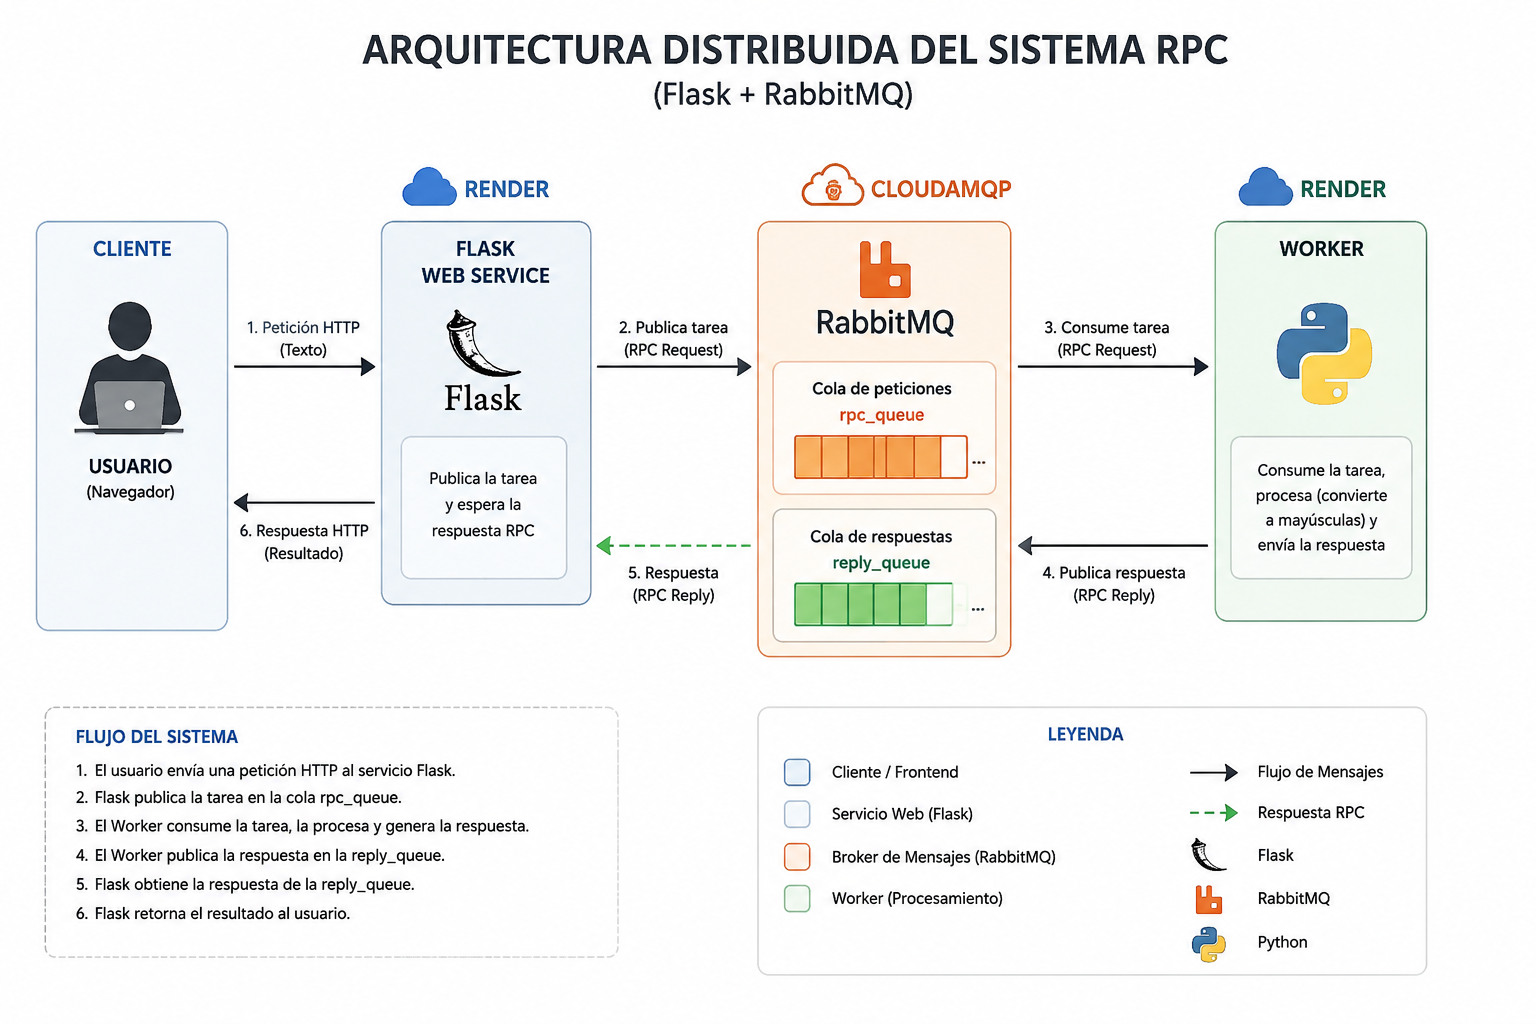
\includegraphics[width=0.85\textwidth]{imagenes/arquitectura.png}
    \caption{Arquitectura distribuida del sistema RPC}
\end{figure}

\section{Requisitos Previos}
Para la correcta ejecución del sistema, asegúrese de contar con:
\begin{itemize}
    \item Python 3.9 o superior.
    \item Una cuenta activa en \href{https://render.com}{Render.com}.
    \item Una instancia gratuita (Little Lemur) en \href{https://cloudamqp.com}{CloudAMQP}.
    \item Herramienta Git instalada.
\end{itemize}

\section{Tecnologías Utilizadas}
\begin{itemize}
    \item Python 3.11
    \item Flask
    \item RabbitMQ
    \item CloudAMQP
    \item Render.com
    \item Gunicorn
    \item AMQPStorm
\end{itemize}

\section{Instalación y Configuración Local}
\subsection{Obtención del código}
\begin{lstlisting}[language=bash]
git clone https://github.com/Victor-Gonzalo-Maldonado-Vilca/Sistemas_Distribuidos_RPC.git
cd Sistemas_Distribuidos_RPC
\end{lstlisting}

\subsection{Entorno de desarrollo}
Cree un entorno virtual para aislar las dependencias:
\begin{lstlisting}[language=bash]
python -m venv venv
# Activar (Linux/Mac)
source venv/bin/activate
# Activar (Windows)
venv\Scripts\activate
\end{lstlisting}

Instale los paquetes requeridos:
\begin{lstlisting}[language=bash]
pip install -r requirements.txt
\end{lstlisting}

\section{Configuración de RabbitMQ (CloudAMQP)}
\begin{enumerate}
    \item Acceda a su panel de CloudAMQP.
    \item Copie la \textbf{AMQP URL}.
    \item Reemplace el valor de la variable \texttt{URL\_NUBE} en los archivos \texttt{worker.py} y \texttt{amqpstorm\_threaded\_rpc\_client.py}.
\end{enumerate}

\section{Despliegue en Render.com}
Para el despliegue en la nube, es crítico configurar dos servicios distintos para permitir el funcionamiento distribuido.

\subsection{Servicio 1: Web Service (Flask)}
\begin{itemize}
    \item \textbf{Build Command:} \texttt{pip install -r requirements.txt}
    \item \textbf{Start Command:} \texttt{gunicorn amqpstorm\_threaded\_rpc\_client:app}
\end{itemize}

\subsection{Servicio 2: Worker}
Debido a las limitaciones del plan gratuito, se despliega como un \textbf{Web Service} configurado para escuchar en el puerto \texttt{10000} (servidor dummy) para evitar que Render detenga el proceso.
\begin{itemize}
    \item \textbf{Start Command:} \texttt{python worker.py}
\end{itemize}

\section{Solución de Problemas}
\begin{itemize}
    \item \textbf{Timeout:} Si recibe un error de tiempo agotado, verifique que el servicio del Worker esté en estado \texttt{Live}. Los servicios gratuitos de Render suelen "dormirse" tras 15 minutos de inactividad.
    \item \textbf{Error de Conexión:} Asegúrese de que la URL de CloudAMQP sea la correcta y que no incluya caracteres extraños.
\end{itemize}
\begin{tcolorbox}[colback=yellow!10]
    Los servicios gratuitos de Render entran en estado de suspensión tras 15 minutos de inactividad.
\end{tcolorbox}
\section{Conclusiones}

\begin{itemize}
    \item Se implementó correctamente un sistema distribuido basado en RPC.
    \item RabbitMQ permitió desacoplar el procesamiento entre cliente y worker.
    \item El despliegue en Render demostró la viabilidad de arquitecturas distribuidas en la nube.
    \item El sistema puede ampliarse fácilmente agregando múltiples workers.
\end{itemize}

\section{Referencias}

\begin{itemize}
    \item RabbitMQ Documentation: \url{https://www.rabbitmq.com/}
    \item Flask Documentation: \url{https://flask.palletsprojects.com/}
    \item Render Documentation: \url{https://render.com/docs}
    \item CloudAMQP Documentation: \url{https://www.cloudamqp.com/docs/}
\end{itemize}
\end{document}
